% Chapter 3

\chapter{CONCEPTUAL FRAMEWORK} % Main chapter title

\label{Chapter3} % Change X to a consecutive number; for referencing this chapter elsewhere, use \ref{ChapterX}

\lhead{Chapter 3. \emph{Conceptual Framework}} % Change X to a consecutive number; this is for the header on each page - perhaps a shortened title

%----------------------------------------------------------------------------------------
%	SECTION 1
%----------------------------------------------------------------------------------------

\section{Research Process}

%\begin{figure}[htbp]
%	\centering
%	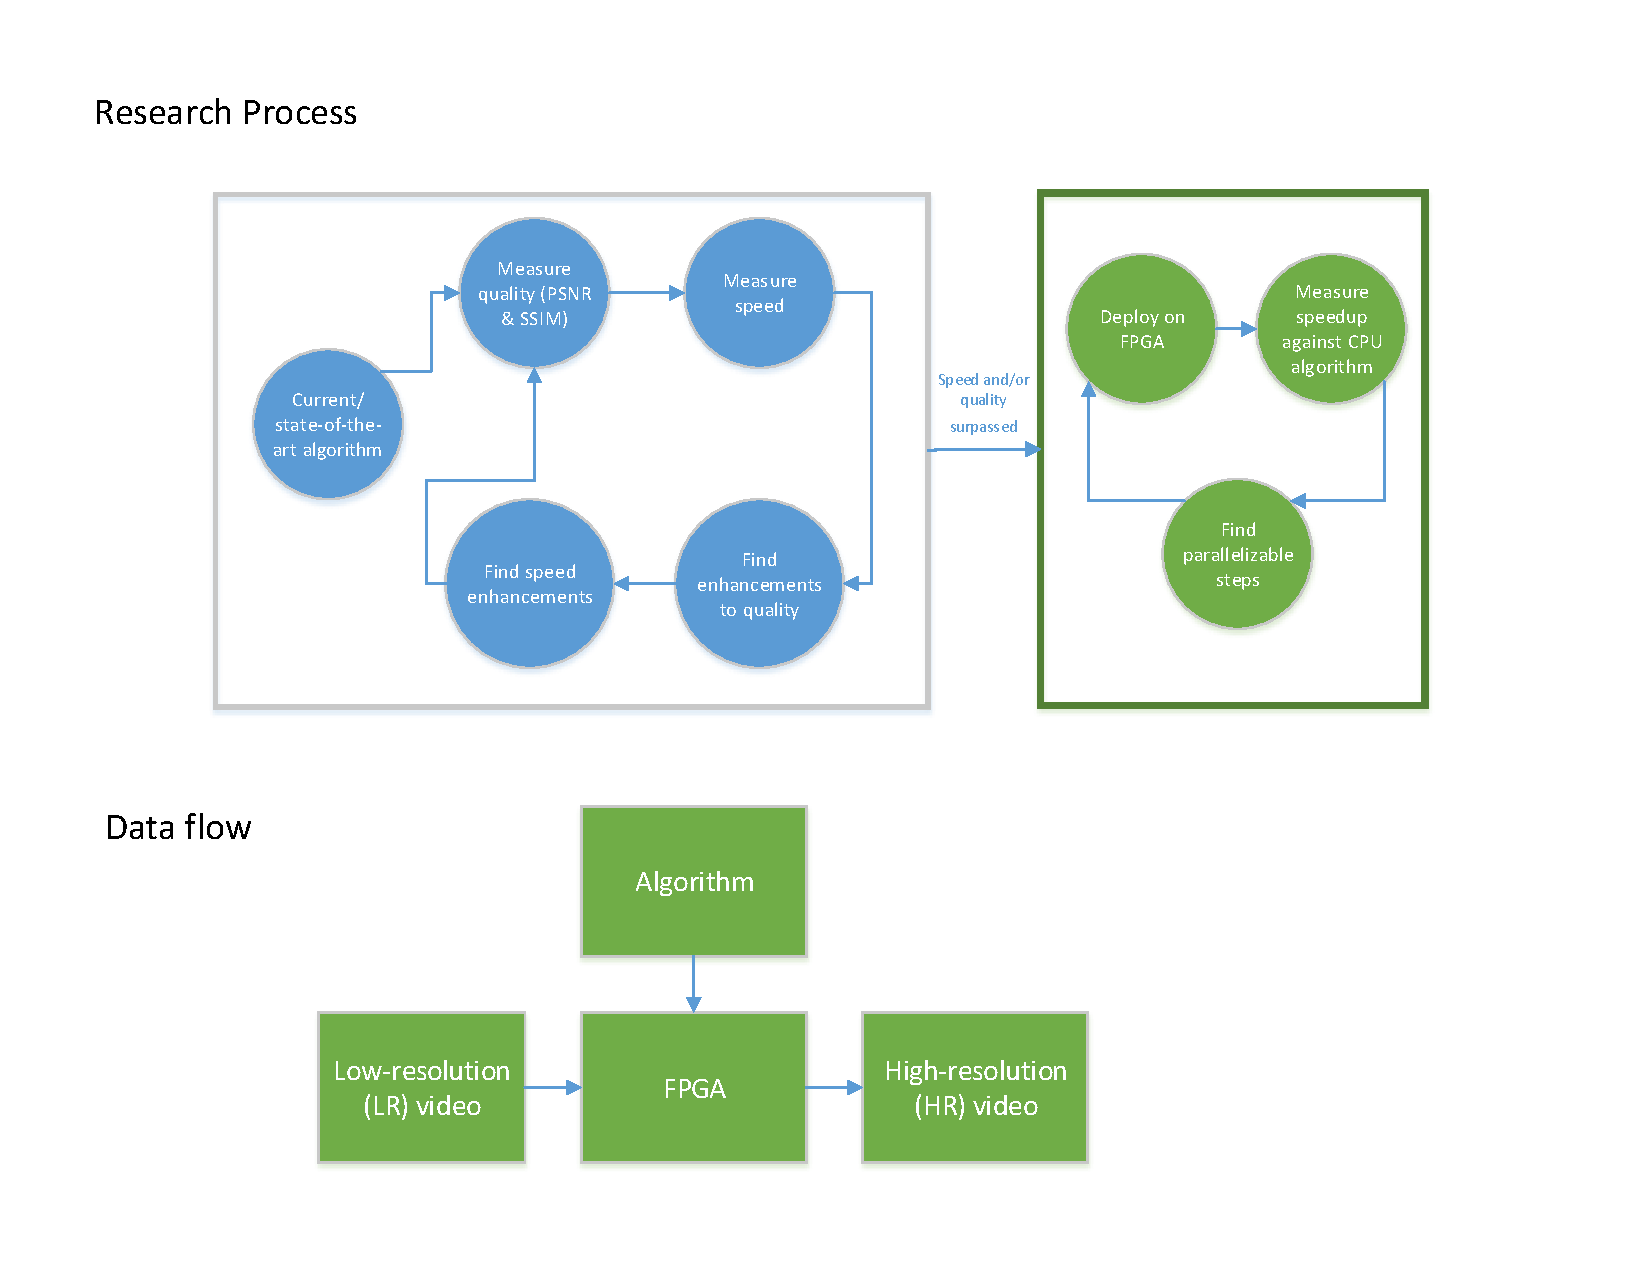
\includegraphics{Figures/framework.pdf}
%	\rule{35em}{0.2pt}
%	\caption[Conceptual Framework]{Conceptual Framework of the Study.}
%	\label{fig:Framework}
%\end{figure}



%-----------------------------------
%	SUBSECTION 1
%-----------------------------------
\subsection{Evaluation of state-of-the-art algorithms}
The m

%-----------------------------------
%	SUBSECTION 2
%-----------------------------------

\subsection{Modifications for speed and quality}


%----------------------------------------------------------------------------------------
%	SECTION 2
%----------------------------------------------------------------------------------------

\subsection{FPGA Deployment and Comparative Tests}

\subsection{Exploiting parallelism for FPGAs}

\section{Data Flow}